\documentclass[a4paper]{article}
\usepackage{listings}
\usepackage{verbatim}
\usepackage{graphicx}
\usepackage{amsmath}
%% Language and font encodings
\usepackage[english]{babel}
\usepackage[utf8x]{inputenc}
\usepackage[T1]{fontenc}
\usepackage{csvsimple}
%% Sets page size and margins
\usepackage[a4paper,top=3cm,bottom=2cm,left=3cm,right=3cm,marginparwidth=1.75cm]{geometry}

\lstset{frame=tb,
  language=Java,
  showstringspaces=false,
  columns=flexible,
  numbers=none,
  commentstyle=\color{green},
  stringstyle=\color{black},
  tabsize=3
}

%% Useful packages
\usepackage{amsmath}
\usepackage{graphicx}
\usepackage[colorinlistoftodos]{todonotes}
\usepackage[colorlinks=true, allcolors=blue]{hyperref}

\begin{document}
\begin{titlepage}
	\raggedleft
	\rule{1pt}{\textheight} 
	\hspace{0.05\textwidth} 
	\parbox[b]{0.75\textwidth}{		
		{\LARGE\bfseries EE - 2703 Applied Programming Lab \\[0.5\baselineskip]  ~\huge Assignment -8}\\[2\baselineskip] 
		{\large\textit{Analysis of Circuits using Symbolic Python}}\\[4\baselineskip] 
		{\Large\textbf{Mohammed Khandwawala}}
        \large EE16B117
		\vspace{0.5\textheight}  
	}

\end{titlepage}


\tableofcontents


\section{Introduction}
This assignment consists of two circuits . One of a Low-Pass filter and a High-Pass filter. The transfer function of the filters from their circuit is obtained by using Symbolic python package. Writing Modified Nodal Analysis Matrix equation to obtain Transfer Function by taking output voltage to input voltage ratio. From the obtained transfer function various analysis in carried out in this assignment.

Some Python functions that are used in this assignment are:
\begin{itemize}
\item \textbf{sym.lambdify}("\textit{symbolic variable name}","\textit{symbolic expression}") - This function converts symbolic expression into lambda function
\item \textbf{sym.simplify}("\textit{symbolic expression}") - This function takes the symbolic expression and return a simplified expression , if not simplified.
\item \textbf{sym.fraction}("\textit{simplified symbolic expression}") - This returns numerator and denominator of the simplified symbolic expression.
\item \textbf{sym.poly}("\textit{"Symbolic expression","symbol"}") - This function takes symbolic expression as input and the symbol/s in the expression and converts it in polynomial.
\item \textbf{polynomial.coeffs()} - This returns the coefficients of the polynomial expression (does not mention the degree)
\end{itemize}
\section{Low-Pass Filter}
The Modified Nodal Analysis matrix obtained on solving the first circuit is given by -
\begin{center}
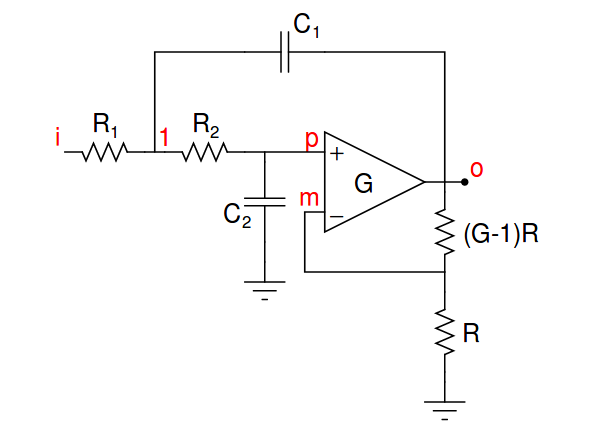
\includegraphics[width=0.8\textwidth]{Selection_001.png}
\end{center}
\begin{gather}
 \begin{bmatrix} 0 & 0 & 1 & \frac{-1}{G} \\  \frac{-1}{1+sR_{2}C_{2}} & 1 & 0 & 0  \\ 0 & -G & G & 1 \\\frac{-1}{R_{1}}+\frac{-1}{R_{2}} - sC_{1} & \frac{-1}{R_{2}} & 0 & sC_{1} \end{bmatrix}
 \begin{bmatrix}
 V_{1} \\ V_{p} \\V_{m}\\V_{o}
 \end{bmatrix}
 =
  \begin{bmatrix}
 0 \\ 0 \\ 0 \\ \frac{V_{i}(s)}{R_{1}}
   \end{bmatrix}
\end{gather}
\subsection{Magnitude Response of Low-Pass Filter}
Defining the function to solve the above matrix equation to obtain the Transfer Function  (Ratio of output to input).
\begin{lstlisting}[language=Python]
def LOWPASS(R1, R2, C1, C2, G, Vi):
	s = symbols('s')
	#Matrix Equations are obtained using modified nodal analysis
	A = Matrix([[0,0,1,-1/G],[-1/(1+s*R2*C2),1,0,0],[0,-G,G,1],[-1/R1-1/R2-s*C1,1/R2,0,s*C1]])
	b = Matrix([0,0,0,-Vi/R1])
	V = A.inv() *b
	return(A,b,V)
\end{lstlisting}

Taking R$_{1}$ = 10K$\Omega$ , R$_{2}$ = 10K$\Omega$, C$_{1}$ = 1nF , C$_{2}$ = 1nF , G = 1.586 and Vi as 1. After obtaining transfer function as a symbolic expression (For Vi = 1 , V$_{o}$ = H(s)) , it is passed to lambdify to get a function that can take return value of the expression. Substituting s by j$\omega$ and sweeping omega logarithmically from 0 to 10$^{8}$.
$$ Vo = \frac{0.0001586}{2.0*10^{-14}s^{2} + 4.414*10^{-9}s + 0.0002}$$
$\omega$$_{o}$(Natural Frequency) = 10$^{5}$ Rad/sec
, Q (Quality Factor) =  0.453
Bandwidth = 56034 Rad/s
\begin{lstlisting}[language=Python]
s = symbols('s')
A,b,V = LOWPASS	(10000.0,10000.0,1e-9,1e-9,1.586,1) 
Vo = V[3] #obtaining expresion of Vout(symbolic)
print Vo
w = p.logspace(0,8,801) #logarithmic range from 0 to 10**8
hf = lambdify(s,Vo,"numpy") #converts symbolic expression to lambda function
t=np.linspace(0,50,1000) #simulating for 50s
ss = 1j*w
v = hf(ss) #substituting s with jw in lambda function equation
\end{lstlisting}
The above obtained response in plotted on a log-log scale.
\begin{lstlisting}[language=Python]
p.loglog(w,abs(v),lw=2)	
p.grid(True)
p.title("|H(jw)| on log-log scale of Low-Pass filter")
p.show()
\end{lstlisting}
The Magnitude response plot of the given filter resembles a Low-Pass filter.
\begin{center}
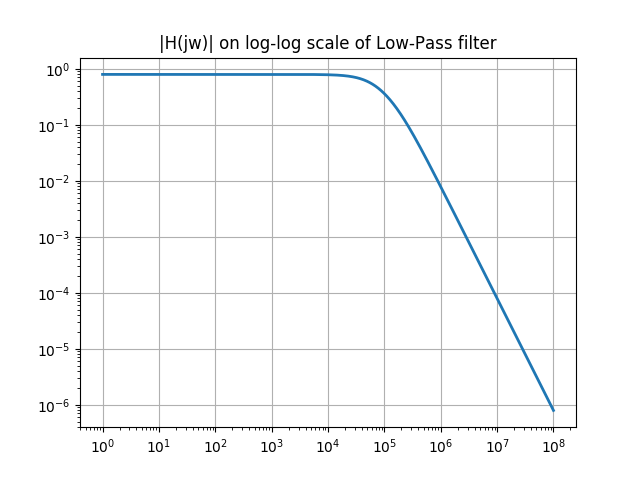
\includegraphics[width=0.8\textwidth]{Figure_1.png}
\end{center}
\subsection{Output of the filter to input sinusoids}
The obtained symbolic expression obtained in the previous part is simplified using  simplify function of python (explained earlier). 
From the simplified transfer function numerator and denominator can be separated using  fraction function. Converting the separated symbolic numerator and denominator expression to polynomial using python function 
Poly and then the coefficients can be extracted to create a polynomial transfer function which can be processed by scipy's signal toolbox.
\begin{lstlisting}[language=Python]
Vo = simplify(Vo)	#simplifying transfer function
NUM,DEN = fraction(Vo)	#saperating numerator and denominator

print Vo

NUM = poly(NUM,s)	#numerator polynomial
DEN = poly(DEN,s)	#denominator polynomial

N = list(NUM.coeffs())	#obtaining the coefficients of numerator polynomial in list
D = list(DEN.coeffs())  #obtaining the coefficients of denominator polynomial in list

\end{lstlisting}
Using signal toolbox function lti we can construct transfer function from the coefficients obtained. For time  3ms we will simulate output for input signal as (sin(2000$\pi$t) + cos(2000000$\pi$t) using lsim.
\begin{lstlisting}[language=Python]
H = sp.lti([float(N[0])],[float(D[0]),float(D[1]),float(D[2])])
t = np.linspace(0,4*10**-3,1000)
Vi = np.sin(2000*np.pi*t) + np.cos(2*10**6*np.pi*t)
t,V_out,svec = sp.lsim(H,Vi,t)
plt.plot(t,V_out) 
plt.grid("True")
plt.title("Output of the Low-Pass filter to input sinusoids (sin(2000$\pi$t) + cos(2000000$\pi$t))")
plt.show()
\end{lstlisting}
The output below clearly shows low-pass response of the filter . Only sinusoid with 1000Hz is visible in the output . Frequency of the sinusoid can be measured from the obtained plot.
\begin{center}
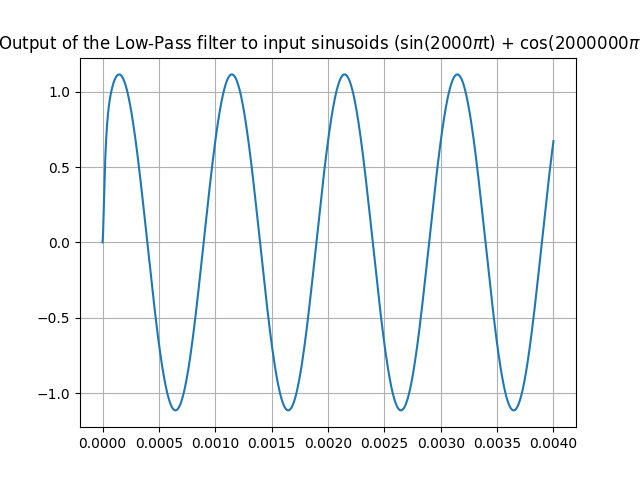
\includegraphics[width=0.8\textwidth]{Figure_2.png}
\end{center}
\subsection{Step Response of a Low Pass Filter}
Step Response of system is output to u(t). We have the Transfer Function of the Low pass Filter. So instead of solving for input 1 V . Already defined function has Vin as a parameter to which $\frac{1}{s}$ can be passed instead on 1.   

\begin{lstlisting}[language=Python]
A,b,V = LOWPASS	(10000.0,10000.0,1e-9,1e-9,1.586,1/s)
Vo = V[3]
w = p.logspace(0,8,801)
hf = lambdify(s,Vo,"numpy")
t=np.linspace(0,50,1000)	
ss = 1j*w
v = hf(ss)
p.loglog(w,abs(v),lw=2)
p.grid(True)
p.title("Step-response of the Low-Pass filter (s - domain)")
p.show()
\end{lstlisting}
The obtained s domain response is shown below.
\begin{center}
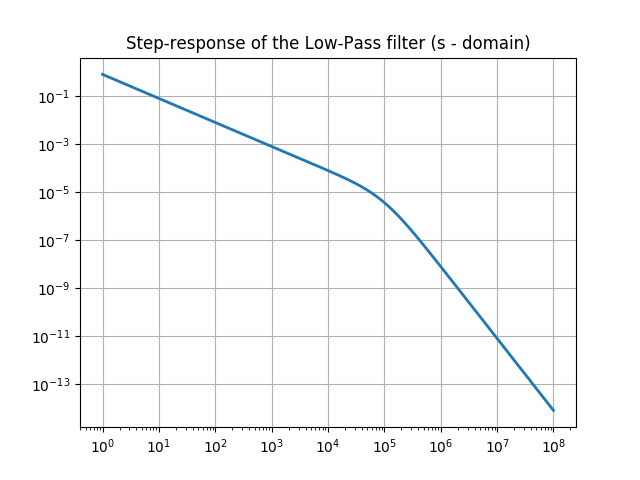
\includegraphics[width=0.8\textwidth]{Figure_6.png}
\end{center}

To obtain the step response in time domain, already obtained polynomial transfer function can be passed u(t) (input as 1 for all t>0) using lsim function .
\begin{lstlisting}[language=Python]
H = sp.lti([float(N[0])],[float(D[0]),float(D[1]),float(D[2])])
t = np.linspace(0,4*10**-3,100000)
Vi = np.ones(100000)
t,V_out,svec = sp.lsim(H,Vi,t)
plt.title("Step-response of the Low-Pass filter (in-time)")
plt.plot(t,V_out) 
plt.grid(True)
plt.show()
\end{lstlisting}
Time domain response to step is shown below in the figure. It falls flat  without ripples because the quality factor of the low pass filter is very low.
\begin{center}
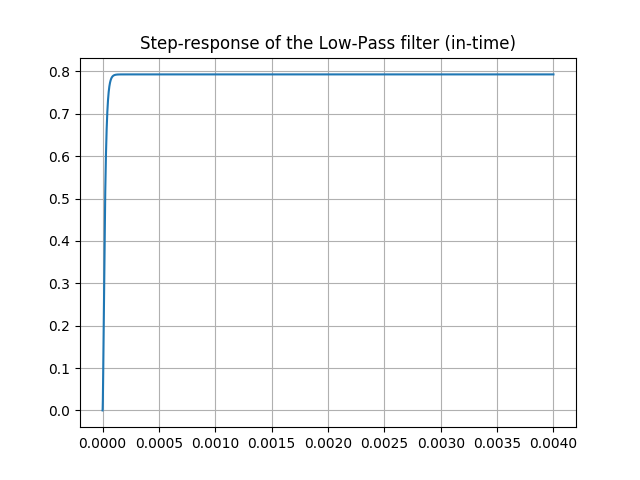
\includegraphics[width=0.8\textwidth]{Figure_8.png}
\end{center}
\section{High-Pass Filter}
The Modified Nodal Analysis matrix obtained on solving the first circuit is given by -
\begin{center}
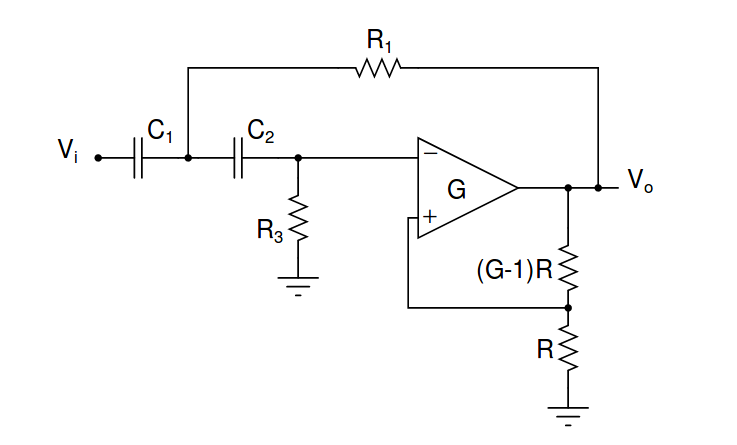
\includegraphics[width=0.8\textwidth]{Selection_002.png}
\end{center}
\begin{gather}
 \begin{bmatrix} 0 & 0 & 1 & \frac{-1}{G} \\  0 & -G & G & 1 \\ \frac{-sC_{2}}{1+sR_{2}C_{2}} & \frac{1}{R_{3}} & 0 & 0   \\\frac{1}{R_{1}}+sC_{1}+sC_{2} & -sC_{2} & 0 & \frac{-1}{R_{1}} \end{bmatrix}
 \begin{bmatrix}
 V_{1} \\ V_{p} \\V_{m}\\V_{o}
 \end{bmatrix}
 =
  \begin{bmatrix}
 0 \\ 0 \\ 0 \\ C_{1}V_{i}s
   \end{bmatrix}
\end{gather}
\subsection{Magnitude Response of High-Pass Filter}
Defining the function to solve the above matrix equation to obtain the Transfer Function  (Ratio of output to input).
\begin{lstlisting}[language=Python]
def HIGHPASS(R1, R3, C1, C2, G, Vi):
	s = symbols('s')
	A = Matrix([[0,0,1,-1/G],[0,-G,G,1],[-s*C2/(1+s*C2*R3),1/R3,0,0],[s*C1+s*C2+1/R1,-s*C2,0,-1/R1]])
	b = Matrix([0,0,0,s*C1*Vi])
	V = A.inv()*b
	return(A,b,V)
\end{lstlisting}

Taking R$_{1}$ = 10K$\Omega$ , R$_{2}$ = 10K$\Omega$, C$_{1}$ = 1nF , C$_{2}$ = 1nF , G = 1.586 and Vi as 1. After obtaining transfer function as a symbolic expression (For Vi = 1 , V$_{o}$ = H(s)) , it is passed to lambdify to get a function that can take return value of the expression. Substituting s by j$\omega$ and sweeping omega logarithmically from 0 to 10$^{8}$.
$$ Vo = \frac{1.586e^{-18}*s^{2}}{2.0*10^{-18}s^{2} + 4.414*10^{-13}s + 2*10^{-8}}$$
$\omega$$_{o}$(Natural Frequency) = 10$^{5}$ Rad/sec
, Q (Quality Factor) =  0.453
and -3dB bandwidth is 17800 Rad/sec
\begin{lstlisting}[language=Python]
s = symbols('s')
A,b,V = HIGHPASS(10000.0,10000.0,1e-9,1e-9,1.586,1)
Vo = V[3]
w = p.logspace(0,8,801)
hf = lambdify(s,Vo,"numpy")
ss = 1j*w
v1 = hf(ss)
\end{lstlisting}
The above obtained response in plotted on a log-log scale.
\begin{lstlisting}[language=Python]
p.loglog(w,abs(v1),lw=2)
p.grid(True)
p.title("|H(jw)| on log-log scale of High-Pass filter")
p.show()
\end{lstlisting}
The Magnitude response plot of the given filter resembles a High-Pass filter.
\begin{center}
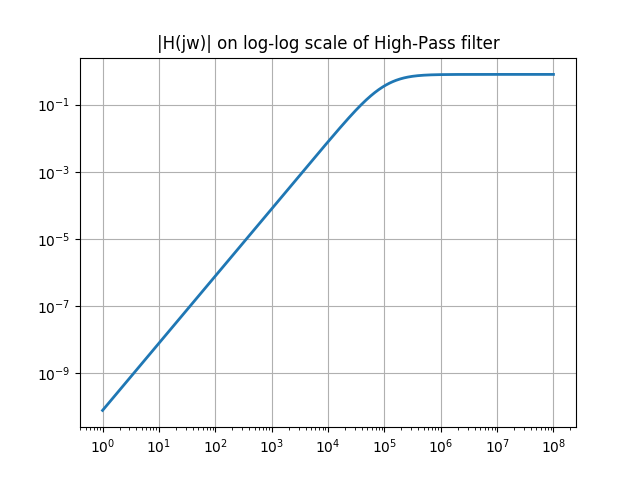
\includegraphics[width=0.8\textwidth]{Figure_3.png}
\end{center}
\subsection{Output of the filter to input sinusoids}
The obtained symbolic expression obtained in the previous part is simplified using  simplify function of python (explained earlier). 
From the simplified transfer function numerator and denominator can be separated using  fraction function. Converting the separated symbolic numerator and denominator expression to polynomial using python function 
Poly and then the coefficients can be extracted to create a polynomial transfer function which can be processed by scipy's signal toolbox.

\begin{lstlisting}[language=Python]
Vo = simplify(Vo)	#simplifying transfer function
NUM,DEN = fraction(Vo)	#saperating numerator and denominator

print Vo

NUM = poly(NUM,s)	#numerator polynomial
DEN = poly(DEN,s)	#denominator polynomial

N = list(NUM.coeffs())	#obtaining the coefficients of numerator polynomial in list
D = list(DEN.coeffs())  #obtaining the coefficients of denominator polynomial in list

\end{lstlisting}
Using signal toolbox function lti we can construct transfer function from the coefficients obtained. For time  3ms we will simulate output for input signal as (sin(2000$\pi$t) + cos(2000000$\pi$t) using lsim.
\begin{lstlisting}[language=Python]
H = sp.lti([float(N[0]),0.0,0.0],[float(D[0]),float(D[1]),float(D[2])])
t = np.linspace(0,4*10**-5,1000)
Vi = np.sin(2000*np.pi*t) + np.cos(2*10**6*np.pi*t)
t,V_out,svec = sp.lsim(H,Vi,t)
plt.plot(t,V_out) 
plt.grid(True)
plt.title("Output of the High-Pass filter to input sinusoids (sin(2000$\pi$t) + cos(2000000$\pi$t))")
plt.show()
\end{lstlisting}
The output below clearly shows High-pass response of the filter . Only sinusoid with 1MHz is visible in the output . Frequency of the sinusoid can be measured from the obtained plot.
\begin{center}
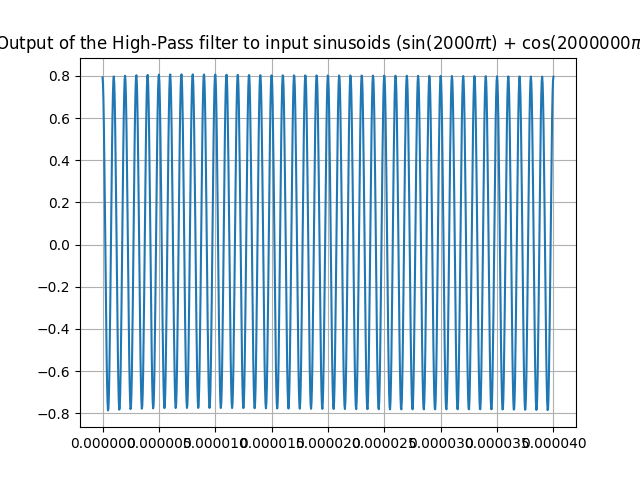
\includegraphics[width=0.8\textwidth]{Figure_4.png}
\end{center}
\subsection{Response of High-Pass filter to damped Sinusoid}
Similar to previous section , the obtained polynomial trasfer function is again used , with the help of python function lsim time domain output to the damped sinusoid is obtained. Sinusoidal input given is $$[sin(2000 \pi t) + cos(2000000\pi t)]e^{-\alpha t}$$
The simulation time is 40$\mu$s and $\alpha$ is chosen to be 100000.
\begin{lstlisting}[language=Python]
H = sp.lti([float(N[0]),0.0,0.0],[float(D[0]),float(D[1]),float(D[2])])
t = np.linspace(0,4*10**-5,1000)
Vi = (np.sin(2000*np.pi*t) + np.cos(2*10**6*np.pi*t))*np.exp(-100000*t)
t,V_out,svec = sp.lsim(H,Vi,t)
plt.plot(t,V_out)
plt.title("High-Pass filters response to damped sinusoid....
...(sin(2000$\pi$t) + cos(2000000$\pi$t))e$^{-100000t}$") 
plt.grid(True)
plt.show()
\end{lstlisting}
The Output of the damped sinusoid to the High Pass filter has a decaying sinusoid of frequency 1MHz ,as the lower frequency components gets highly attenuated.
\begin{center}
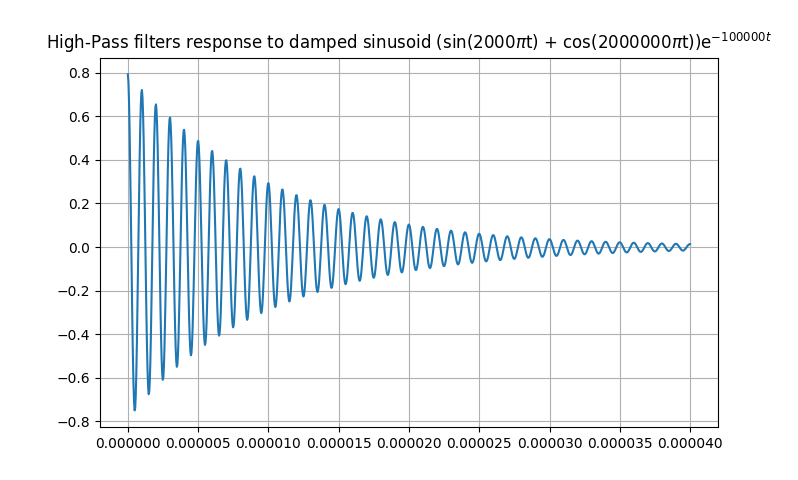
\includegraphics[width=0.8\textwidth]{Figure_5.png}
\end{center}
\subsection{Step Response of a High-Pass Filter}
Step Response of system is output to u(t). We have the Transfer Function of the High pass Filter. So instead of solving for input 1 V . Already defined function has Vin as a parameter to which $\frac{1}{s}$ can be passed instead on 1.   

\begin{lstlisting}[language=Python]
A,b,V = HIGHPASS(10000.0,10000.0,1e-9,1e-9,1.586,1/s)
Vo = V[3]
w = p.logspace(0,8,801)
hf = lambdify(s,Vo,"numpy")
ss = 1j*w
v1 = hf(ss)
p.loglog(w,abs(v1),lw=2)
p.grid(True)
p.title("Step-response of the High-Pass filter (s - domain)")
p.show()

\end{lstlisting}
The obtained s domain response is shown below. It is a band pass filter as integrating a High pass filter gives a band-pass filter.
\begin{center}
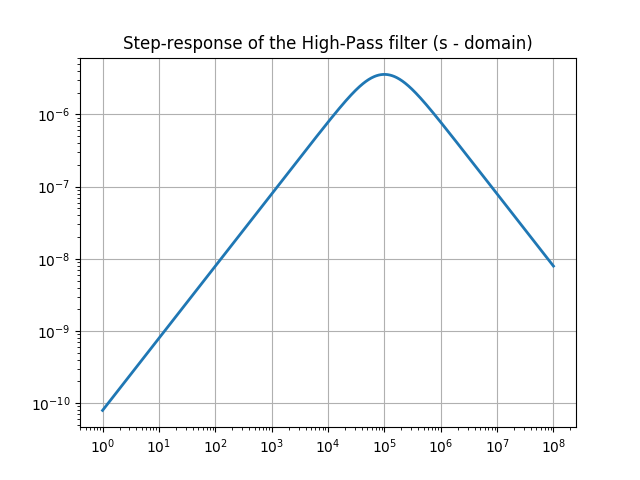
\includegraphics[width=0.8\textwidth]{Figure_9.png}
\end{center}

To obtain the step response in time domain, already obtained polynomial transfer function can be passed u(t) (input as 1 for all t>0) using lsim function .
\begin{lstlisting}[language=Python]
H = sp.lti([float(N[0]),0.0,0.0],[float(D[0]),float(D[1]),float(D[2])])
t = np.linspace(0,4*10**-3,100000)
Vi = np.ones(100000)
t,V_out,svec = sp.lsim(H,Vi,t)
plt.title("step response of the High-Pass filter (in-time)")
plt.grid(True)
plt.plot(t,V_out) 
plt.show()
\end{lstlisting}
Time domain response to step is shown below in the figure. It falls flat  without ripples because the quality factor of the High pass filter is very low.
\begin{center}
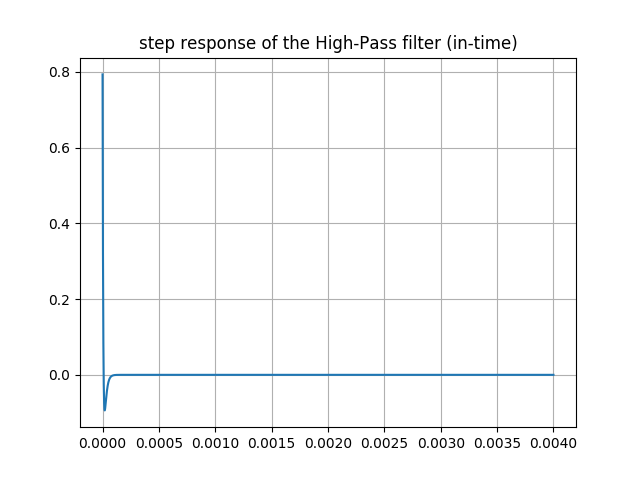
\includegraphics[width=0.8\textwidth]{Figure_10.png}
\end{center}
\end{document}

